\section{\texorpdfstring{ Ethical and Legal
Issues}{ Ethical and Legal Issues}}\label{ethical-and-legal-issues}

A man without ethics is a wild beast loosed upon this world.---Albert
Camus

In your professional career you are going to face ethical dilemmas, and
how you respond to them will affect your reputation, your employability,
and the welfare of others. Systems are developed for use by other
people, and the decisions that go into their design impacts the health
and safety of those people. There are plenty of high profile examples,
such as the two space shuttle disasters, that make it clear that the
decisions of engineers and scientists have serious implications. Beyond
issues in the technical aspects of design, there are professional ethics
that govern the broad scope of interactions between people in the
workplace. The aim of this chapter is to present the basics of
engineering ethics and provide guidance for addressing dilemmas when
they arise. It presents a basic overview of morality and ethics,
professional codes that apply to the engineering profession,
intellectual property and legal issues as they relate to design, how to
apply ethics throughout the design process, and guidance for handling
ethical dilemmas. The chapter concludes with case studies that provide
an opportunity to apply ethical decision-making skills.

Learning Objectives

By the end of this chapter, the reader should:

\begin{itemize}
\item
  Understand what is meant by morals, ethics, and values.
\item
  Be familiar with the IEEE Code of Ethics.
\item
  Understand what a patent is, the criteria for filing for one, and the
  elements that constitute it.
\item
  Understand the difference between patents, trade secrets, and
  copyrights.
\item
  Understand the concepts of negligence and strict liability as they
  apply to product design.
\item
  Understand how to incorporate ethical issues throughout the design
  process.
\item
  Be able to analyze ethical case studies and suggest solutions to the
  dilemmas that they embody.
\end{itemize}

\subsection{Ethical Theory in a
Nutshell}\label{ethical-theory-in-a-nutshell}

Here is an ethical dilemma to consider as we start our discussion. Let's
assume that you are conducting a job search during your senior year in
college and have interviewed with several prospective employers. Company
A offers a you job and you accept the position and you sign a contract
agreeing upon a starting salary, position, and start date. Two weeks
later, Company B also offers you a job with a higher starting salary and
work that you find personally more interesting. You have a choice to
make. Do you turn down the offer of Company B and stay with A? Or do you
accept the offer made by B and then inform A that you are not going to
work for them? This is a classic dilemma that many students will face,
and rather than trying to answer it now, let's revisit it later.

There is often confusion as to what exactly is meant by the related
concepts of \emph{\textbf{ethics}} and \emph{\textbf{morals}}. Morality
is concerned with principles of right and wrong and the decisions that
derive from these principles. Morals are often taught by stories that
are common in all cultures, such as Aesop's fable of the boy who cried
wolf. In this story, the boy was watching sheep and cried wolf when
there was no wolf present. In response, all of the villagers came
running to help him, only to find no wolf. When the wolf did later
appear and the boy cried for help once again, nobody believed him nor
came to help, and the wolf scattered the flock. The moral of this story
is that it is wrong to lie, and when a person becomes known as a liar,
nobody will believe him/her even if he/she is telling the truth.

The term ethics is closely related to morals and they are often used
interchangeably. According to the \ul{American Heritage Dictionary},
ethics is defined as:

\begin{quote}
1. Branch of philosophy that deals with the general nature of good and
bad and the specific moral obligations of and choices to be made by the
individual in her/his relationship to others. 2. Rules or standards
governing conduct, especially those of a profession.
\end{quote}

Ethics is the philosophy or study of moral obligations and the choices
to be made by individuals. It is important to understand that if there
is no decision to be made, there is no ethical dilemma. The choices to
be made are based upon a belief as to what is good or bad, and the
decisions must impact relationships to others.

Morals derive from \emph{\textbf{principles,}} which are fundamental
laws or rules that govern behavior. An example of a principle is the
Golden Rule, which states that people should treat others as they
themselves would like to be treated. The Golden Rule is a universal
principle and embodied in one form or another in all major religions and
belief systems of the world. Another example of a principle is the
belief that people should be honest and trustworthy in their dealings
with others. Value is another term that is often heard in ethical
discussions. A \emph{\textbf{value}} is something that a person or group
believes to be valuable or worthwhile. This could be relatively
innocuous such as valuing baseball as a sport, or something more
significant such as valuing hard work. A group of thieves may believe
that it is valuable to steal from other people, but not from their own
group. As these examples show, shared values may be good or bad. The
final example clearly violates the principles of the Golden Rule and is
considered bad by most people.

\textbf{\emph{Rule-based ethics}} are based upon a set of rules that can
be applied to make decisions. In the strictest form they are considered
to be absolute in terms of governing behavior---either you follow the
rule (good) or break the rule (bad). This type of an ethical system is
based upon the principles of \emph{universality} and
\emph{transitivity}. Universality means that the governing rules are
such that they can be accepted by everyone, while transitivity means
that you would accept others applying the same decision to you. A
problem with rule-based ethics is defining a universal set of rules that
everyone can agree upon. There may be a few rules or principles that can
be agreed upon by all, but going beyond that is difficult.

\emph{\textbf{Conditional rule-based ethics}} means that there are
certain conditions under which an individual can break a rule. This is
generally because it is believed that the moral good of the situation
outweighs the rule. For example, if you have a seriously injured person
in your car and are transporting them to the hospital, is it acceptable
to exceed the speed limit? In this case, it may be deemed that the moral
good of getting the person prompt medical attention outweighs the
obligation to obey the speed limit. It is generally believed that
killing others is wrong, except in the case of war. Is it acceptable to
cheat on an exam because you stayed up all night to help your sick
roommate? Or is it acceptable to cheat because you simply did not have
enough time to study because of your other obligations? In each of these
cases a moral choice has to be weighed.

In \emph{\textbf{utilitarian ethics}}, decisions are made based upon the
decision that brings about the highest good for all, relative to all
other decisions. This sounds appealing, but has drawbacks in that bad
choices may need to be made for certain parties in order to achieve this
overall good. It becomes very difficult to determine exactly what the
highest good is. \emph{\textbf{Situational ethics}} are where decisions
are made based on whether they produce the highest good for the person.
In this case, decisions are made based upon the impact to the individual
and situation at hand. This is generally considered a poor ethical
decision-making approach.

Let's conclude this section with a new scenario. Let's assume that you
are conducting a job search and Company A offers you a job, you agree
upon terms of the offer, accept it, and sign a contract. You then inform
the other companies that interviewed you that you are no longer
available. One month later Company A calls you and notifies you that
they are rescinding their offer. Although they can no longer offer you
the job, they will provide you with \$1,000 in compensation for
rescinding the offer. You later find out that Company A just offered the
exact same job to another student in your class who has a higher grade
point average than yours and more experience with the technical products
they design. Was the decision of the company ethical? Returning to the
original case, is it ethical for the student to rescind their acceptance
of the original job offer and then accept the other?

\subsection{The IEEE Code of Ethics}\label{the-ieee-code-of-ethics}

Most engineering disciplines have associated with them a professional
society or organization. In electrical and computer engineering two
important ones are the Institute of Electrical and Electronics Engineers
(IEEE) and the Association for Computing Machinery (ACM). The objective
of professional societies is to promote and support their respective
fields. They offer a variety of services and benefits to their members,
such as access to technical information, networking opportunities, and
financial services. They also define accepted practices of their members
that are embodied in an ethical code. In fact, professional societies
were originally created to provide guidance for ethical practices in
their field and to ensure the safety of the public. The IEEE Code of
Ethics, shown in Table 11.1, applies broadly to the electrical,
computing, and software fields.

\textbf{Table 11.1} The IEEE Code of Ethics.

\textbf{We, the members of the IEEE,} in recognition of the importance
of our technologies in affecting the quality of life throughout the
world, and in accepting a personal obligation to our profession, its
members and the communities we serve, do hereby commit ourselves to the
highest ethical and professional conduct and agree:

1. to accept responsibility in making engineering decisions consistent
with the safety, health and welfare of the public, and to disclose
promptly factors that might endanger the public or the environment;

2. to avoid real or perceived conflicts of interest whenever possible,
and to disclose them to affected parties when they do exist;

3. to be honest and realistic in stating claims or estimates based on
available data;

4. to reject bribery in all its forms;

5. to improve the understanding of technology, its appropriate
application, and potential consequences;

6. to maintain and improve our technical competence and to undertake
technological tasks for others only if qualified by training or
experience, or after full disclosure of pertinent limitations;

7. to seek, accept, and offer honest criticism of technical work, to
acknowledge and correct errors, and to credit properly the contributions
of others;

8. to treat fairly all persons regardless of such factors as race,
religion, gender, disability, age, or national origin;

9. to avoid injuring others, their property, reputation, or employment
by false or malicious action;

10. to assist colleagues and co-workers in their professional
development and to support them in following this code of ethics.

\emph{Approved by the IEEE Board of Directors, August 1990}

Some of the values embodied in the code are that of treating others with
fairness and respect (8--10), honesty and trustworthiness (2--4), and
professional competence (6--7). The importance of the safety of the
public is clearly identified in the first and ninth items of the code.
The code provides a common basis for analyzing ethical cases studies and
is applied for these purposes in subsequent sections.

\subsection{Intellectual Property and Legal
Issues}\label{intellectual-property-and-legal-issues}

It is important to understand some legal issues, particularly as they
impact product design and development. The first considered is
intellectual property, which seeks to answer the question of who owns an
idea or invention. The second is that of legal liability, which comes
into play if somebody is injured or harmed by a product or system.

\subsubsection{Intellectual Property}\label{intellectual-property}

The intent of designing a new product is usually to sell it for a
profit, which leads to the issue of ownership of both the intellectual
property and the profits. The tools for protecting intellectual property
are patents, trade secrets, and copyrights. Be aware that when you enter
the workforce as an engineer, your employer may ask you to sign an
agreement assigning their company rights to all of the intellectual
property that you create while in their employ. Such contracts are
common and enforceable.

The most well-known way of protecting a design or invention is with a
\emph{\textbf{patent}}. If a patent is held for a technology, others
cannot use it without permission of the owner. The owner can deny others
the right to use it, or grant the right to use it in exchange for
monetary compensation. The two types of patents are utility and design
patents. The United States Patent and Trademark Office (USPTO) defines
the difference between the two as follows:

\begin{quote}
A utility patent may be granted to anyone who invents or discovers any
new and useful process, machine, article of manufacture, compositions of
matter, or any new useful improvement thereof. A design patent may be
granted to anyone who invents a new, original, and ornamental design for
an article of manufacture.
\end{quote}

The one that is of most interest for this discussion is the utility
patent, as the design patent focuses on aesthetic design issues.

In order to be granted a utility patent, the invention must meet three
conditions: it must be novel, non-obvious, and useful. Novelty means
that the idea must be new and that nothing like it already exists. It
cannot be an idea that is already patented or has been published for
more than a year. The non-obvious condition means that another person
would not be expected to develop the same idea based upon existing
technology. As an example, for personal computers, it would not be
possible to patent the idea of increasing data storage by adding
multiple disk drives, since this is an obvious extension of existing
technology. Useful means that the device must perform a useful function
and be able to be reduced to practice. You could not patent the concept
for a transporter of the type seen on science fiction shows, such as
\emph{Star Trek}, where people are beamed instantaneously through space
from one place to another---unless of course you can reduce it to
practice.

To a file a patent, extensive research needs to be done to be sure that
the idea is novel. A good place to start is the US Patent Trademark
Office (USPTO) website (\href{http://www.uspto.gov}{www.uspto.gov}) and
its searchable database of patents back to 1790. The database allows
full text search of patents from 1976 forward and patent number search
back to 1790. It provides full images of all patents in the database.
The website also has information on how to apply for a patent and
describes the differences between patents, trademarks, and copyrights.
The elements that are contained in a patent are:

\begin{itemize}
\item
  \emph{A citation of prior art}. This is similar patents and publicly
  reported technology.
\item
  \emph{A description of the invention}. This describes how it operates
  and how it would be reduced to practice.
\item
  \emph{Claims}. They are the legal description of the invention and its
  unique aspects.
\end{itemize}

The claims are used to determine if another party is infringing upon a
patent, and thus they must be carefully thought out and properly worded.
If the claims are too broad or too specific then they may not provide
much protection. There are fees for filing the patent and for periodic
maintenance that can cost between \$5,000 and \$10,000 over the life of
the patent. Hiring a good patent attorney is invaluable in the
application process and will cost money---it is not unusual to spend
\$20,000 for lawyer and application fees. When selecting a patent
attorney, make sure that he/she has a good track record and reputation.

An example patent for a hardware design of a fast floating point
overflow and sign detection unit (US Patent \#6,779,013) is shown in
Figure 11.1. The patent is owned by Intel Corporation and the inventor
was one of their employees. The first page identifies prior art that
relates to this patent. This includes previous patents related to this
technology, which in this case goes back to 1991. It is not unusual to
cite prior patents that go back 50 or 100 years. In addition to patents,
prior art in publicly available literature is identified. The first page
also identifies the number of claims and supporting figures, and shows
the high-level design architecture. A description of the system starts
on the second page as shown in Figure 11.1 (b). The complete description
is fairly lengthy and only the first page is shown. It is similar to a
technical report in that it provides background on the technology and
describes the invention and its operation in detail. The final page of
the patent (Figure 11.1 (c)) identifies the legal claims that make the
invention unique.

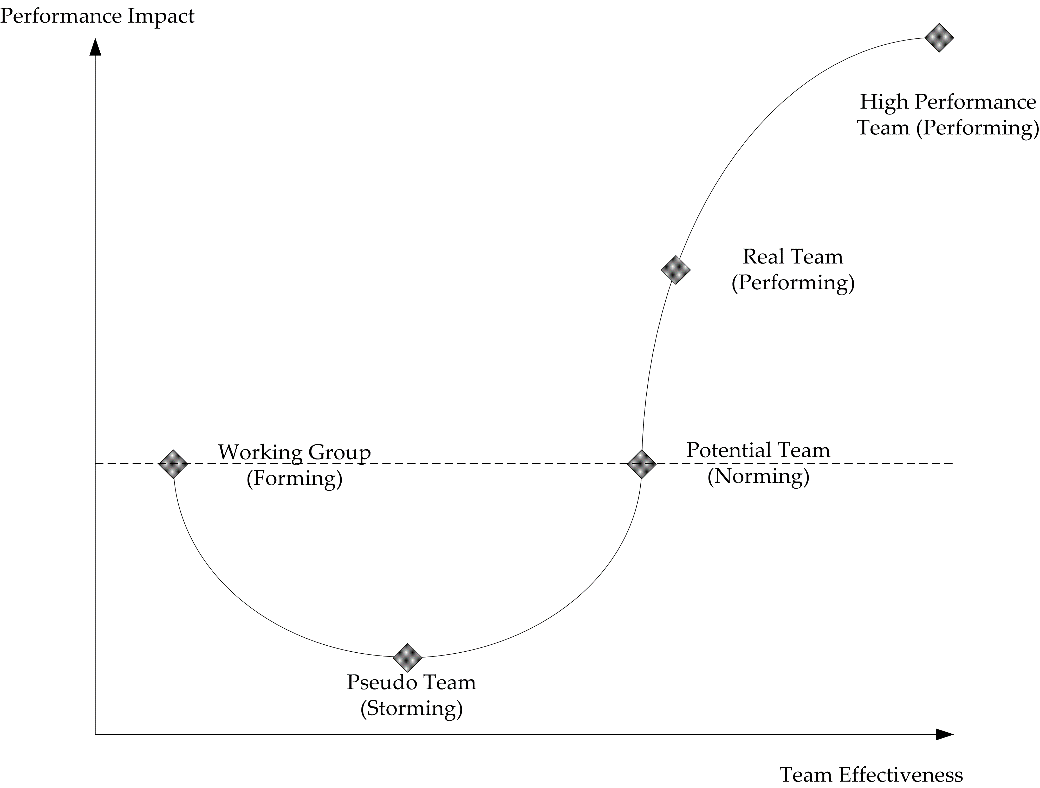
\includegraphics[width=4.69792in,height=7.23958in]{media/image1.png}

\textbf{Figure 11.1} (a) Example of a US patent for a floating point
overflow and sign detection unit.

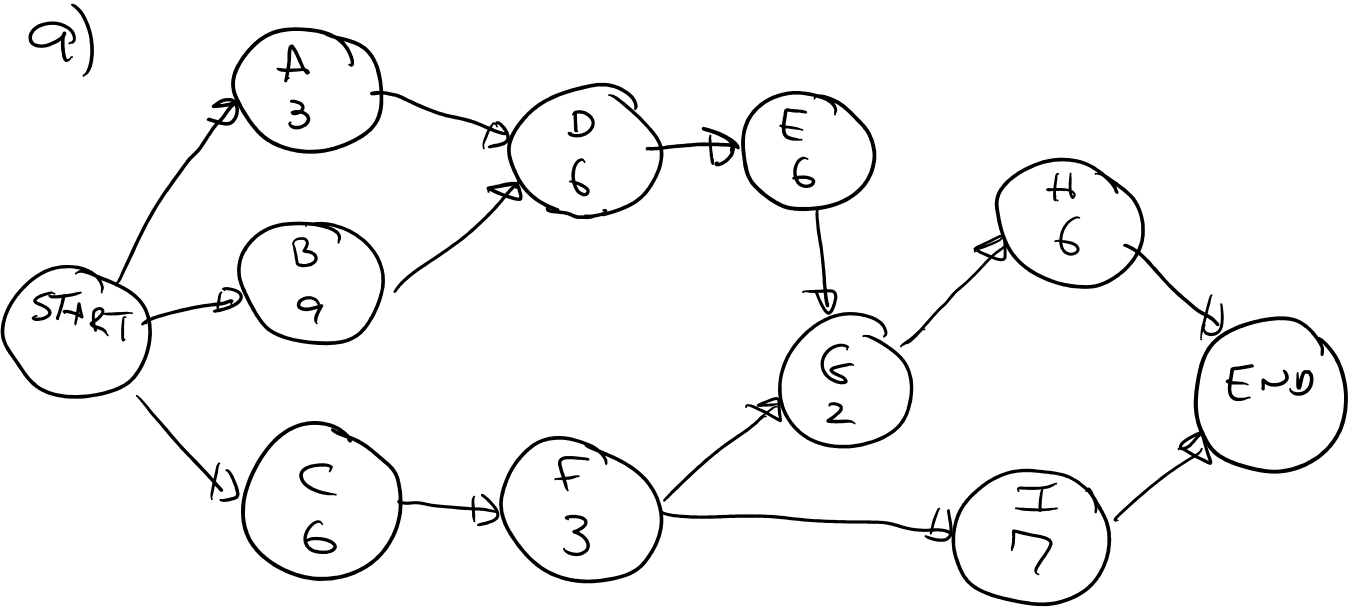
\includegraphics[width=4.70833in,height=7.26042in]{media/image2.png}

\textbf{Figure 11.1} (b) First page of the patent description.

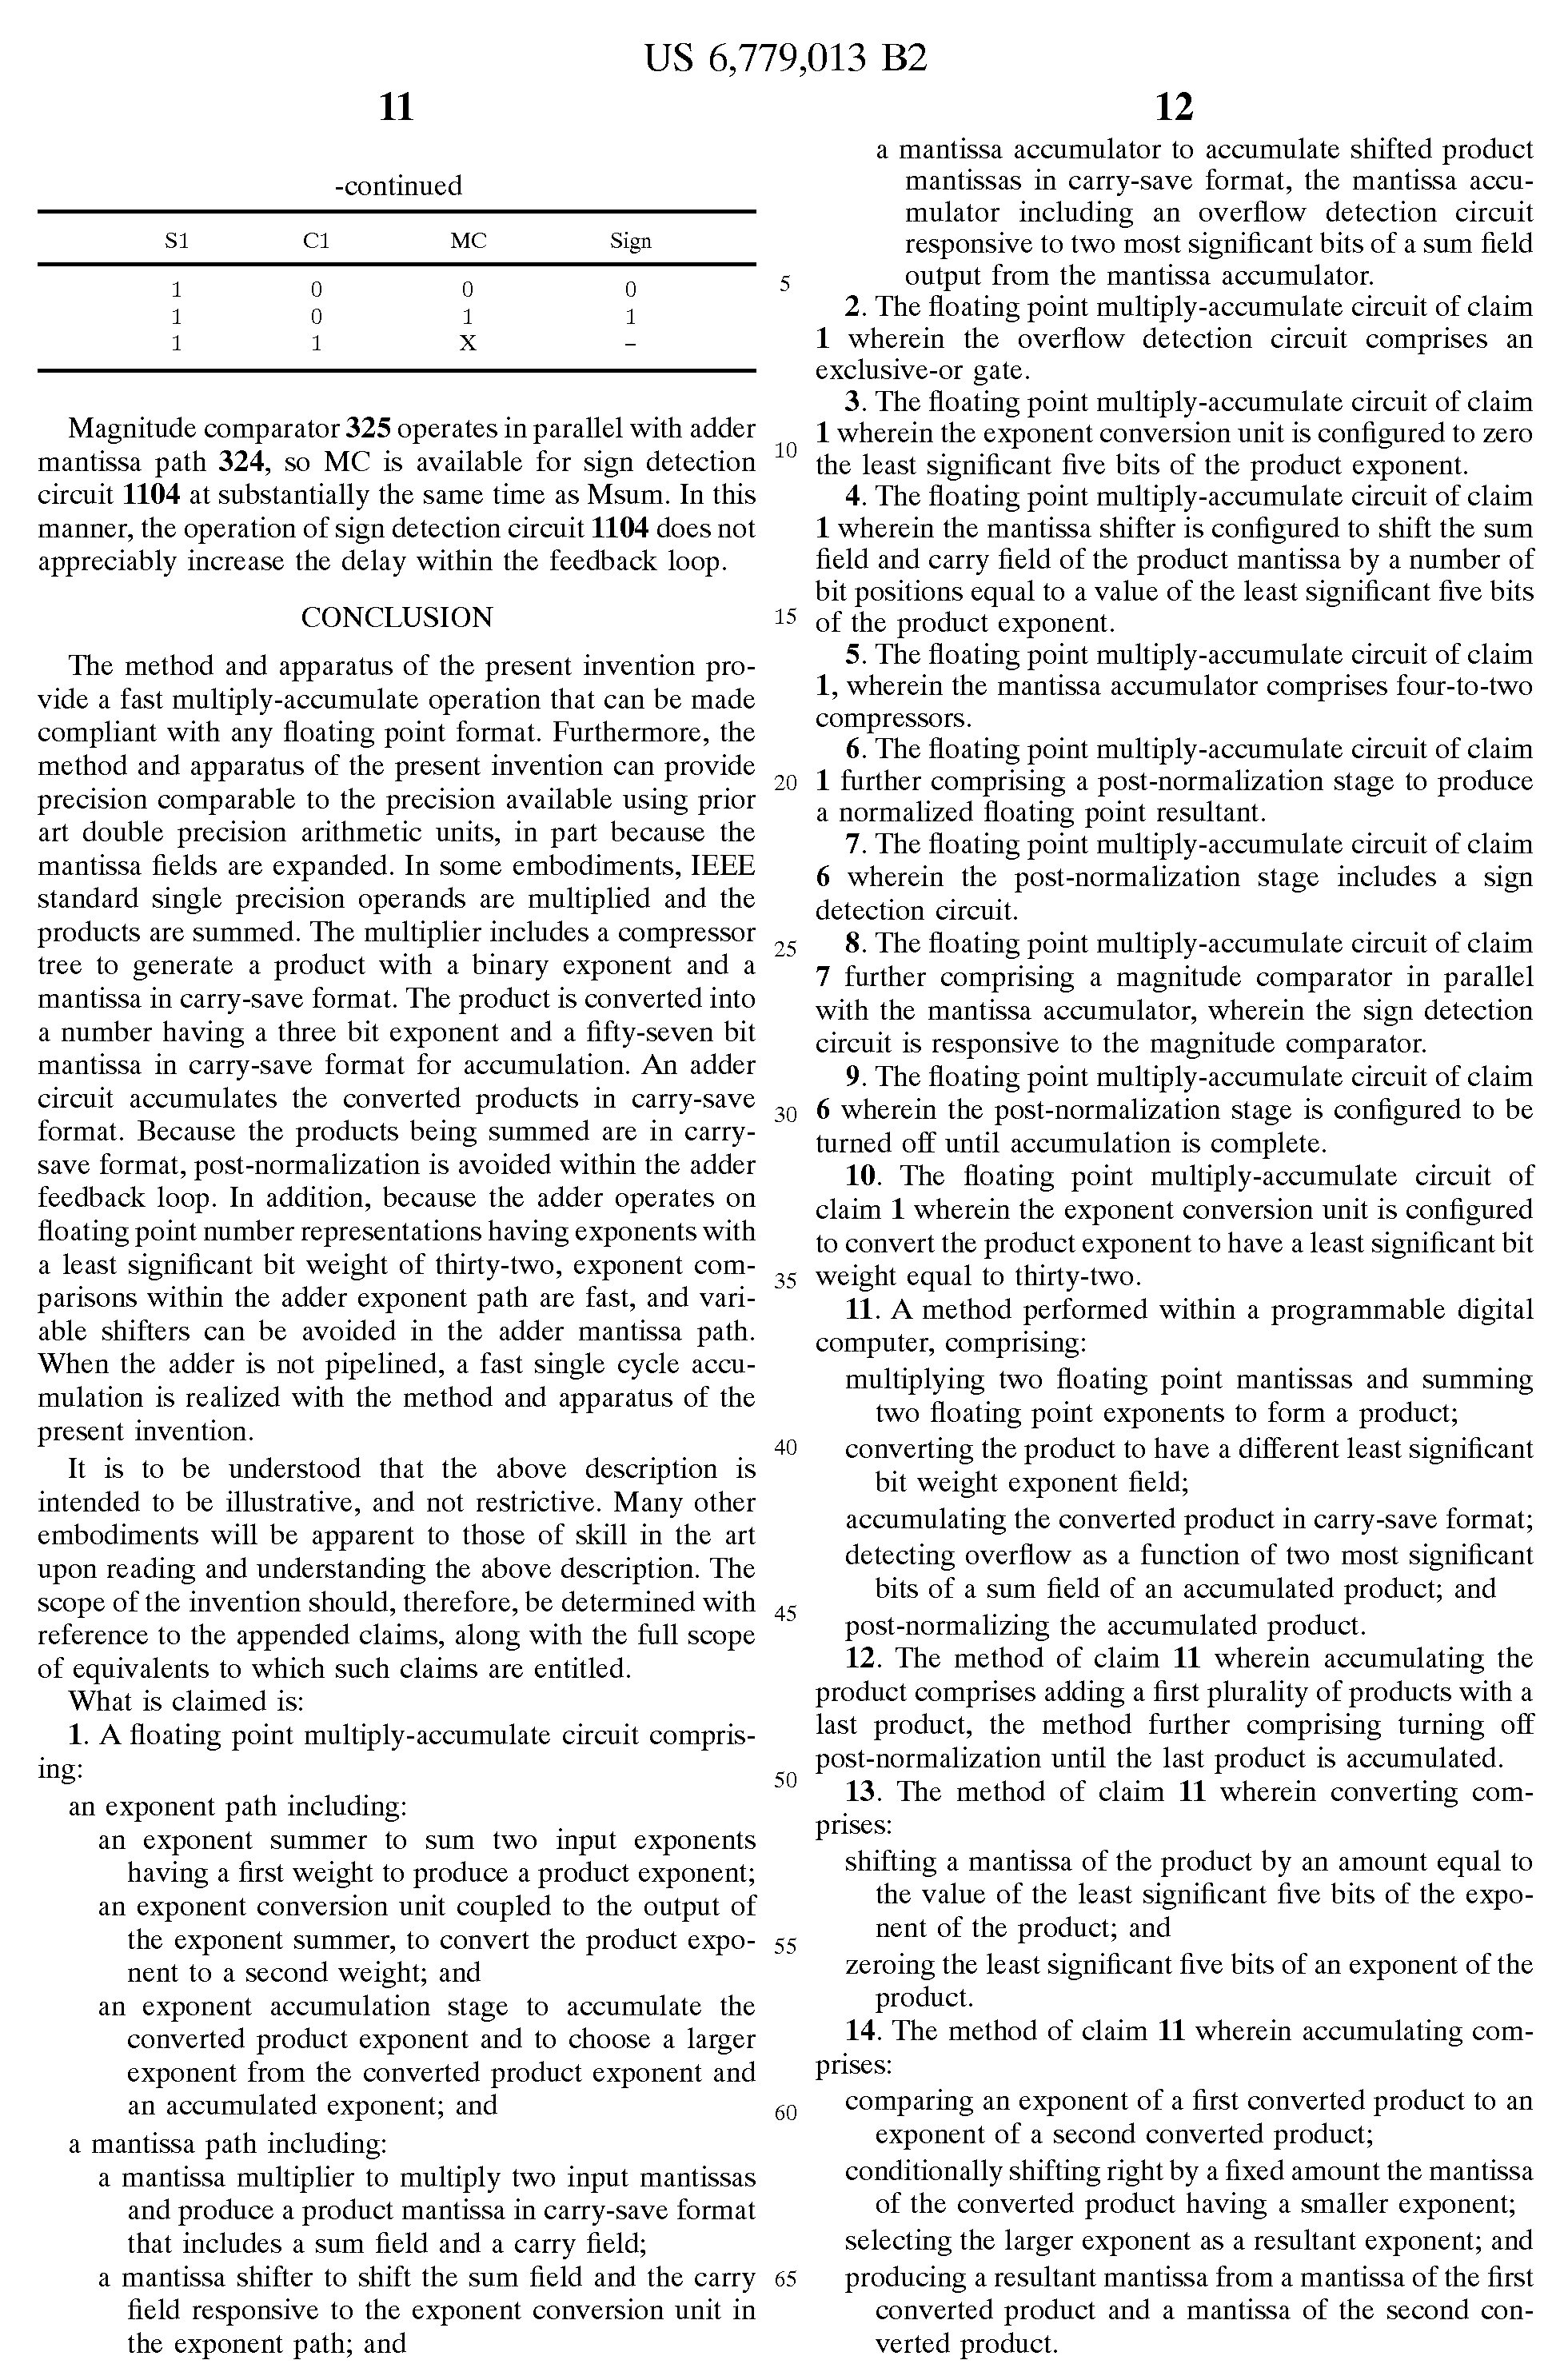
\includegraphics[width=4.79167in,height=7.25in]{media/image3.png}

\textbf{Figure 11.1} (c) Conclusion of the patent and its claims.

In the United States, patents are granted based upon the concept of
first to conceive the invention, not first to file the patent
application. If two parties are applying for a patent at the same time,
then the one who demonstrates that they were the first to conceive the
idea and reduce it to practice receives the patent. Good records must be
maintained to prove this. It is done by recording inventions in a bound
design notebook with numbered pages that cannot be removed. All entries
should be clearly described, understandable by other engineers, and be
signed and dated. For the best protection, entries should be signed and
witnessed by at least one other person and the notebook should be
occasionally notarized. Pages should not be removed from the notebook
and entries should be made in non-erasable pen. Mistakes and blank
spaces should be crossed out, signed, and dated. Figures should be drawn
directly in the notebook, while computer generated figures are pasted in
so that they are not removable. It is good practice to maintain a design
notebook even if you are not planning to patent your ideas.

Once a patent is granted, it is good for 20 years---after it expires,
the invention is fair game for anybody to use. Let's assume that you are
the owner of a patent and you find that somebody is infringing upon it.
Is the government going to come in and start legal action against the
infringer? No---a patent only gives the owner a right to sue others if
they infringe upon it. The government does not actively seek out
offenders and protect your intellectual property. The owner of the
patent must protect it.

There are drawbacks to patents. The owner must be vigilant in defending
a patent and may have to initiate legal action to do so. Once an idea is
patented, it is made public for all to see on the government's website.
This may not be a good idea depending upon the technology and
competitive situation. An alternative that many companies employ to
protect intellectual property is to hold them as \emph{\textbf{trade
secrets}}. Obviously, the idea must be kept secret so that others cannot
find out about it. This is often done by restricting the number of
people who have access to the idea and by having those who do know about
it sign a \emph{\textbf{non-disclosure agreement.}} It is common
practice for companies to ask employees and visitors to their facilities
to sign a non-disclosure agreement that prevents the signer from
disseminating information about their products, services, and trade
secrets. If one breaks a non-disclosure agreement, they can be held
legally liable. Trade secrets pose another type of risk to a company,
since once the secret is revealed, it is fair game for competitors. One
way to determine a competitor's trade secrets is through the use of
\emph{\textbf{reverse-engineering,}} where a device or process is taken
apart to understand how it works. Reverse-engineering is legal if the
information is obtained through legal means, but one must be careful
with the information that is obtained and not copy it unless legally
allowed to do so. The Digital Millennium Copyright Act of 2000 prohibits
breaking technological protections, such as encryption, to learn about a
competitor's product.

\emph{\textbf{Copyrights}} protect published works such as books,
articles, music, and software. A copyright means that others cannot
distribute copyrighted material without permission of the owner. It is
easy to obtain a copyright---all that a person has to do to copyright
material is indicate the word ``copyright'' on the work, along with the
year of publication, and identify the name of the copyright holder.
Copyrights can be officially registered through the US Copyright Office,
and it is a good idea to do so for involved works such as writing a book
or publishing music. Registering provides a stronger legal basis for
pursuing claims. Copyrights are good for the lifetime of the holder plus
50 years, while for a company they are good for 75 years.

\subsubsection{Liability and Negligence}\label{liability-and-negligence}

Civil lawsuits, which are those that are relevant for our discussion,
are those in which one party sues another. They involve something that
is known as a \emph{\textbf{tort,}} which serves as grounds for the
lawsuit. A tort is a wrongful act, though not necessary illegal, for
which a civil lawsuit can be brought, including product liability. A
company or person can be sued for damages caused by a product design and
be held \emph{\textbf{liable}} for them, meaning required to pay
monetary damages.

The two standards for determining legal liability in tort law are that
of negligence and strict liability. In the case of
\emph{\textbf{negligence,}} it must be shown that the manufacturer did
not follow reasonable standards and rules that apply to the situation
and also committed a wrongful act. Exactly what constitutes reasonable
has to be determined for the particular case. For a product design, a
manufacturer can be held legally liable for negligence if the plaintiff
demonstrates that the following four conditions hold true:

\begin{enumerate}
\def\labelenumi{\arabic{enumi}.}
\item
  The manufacturer had a duty to follow reasonable standards and rules.
\item
  There was a breach of duty (i.e., failed to include safety devices).
\item
  The plaintiff was harmed.
\item
  The breach caused the harm.
\end{enumerate}

Depending on the severity of the danger, there are different levels of
negligence: simple, gross, and criminal. Negligence claims can be
brought for design flaws, manufacturing defects, and for failing to warn
the user of safety hazards.

An even less stringent standard than negligence is known as
\emph{\textbf{strict liability}}, in which the following four conditions
must hold true:

\begin{enumerate}
\def\labelenumi{\arabic{enumi}.}
\item
  The product was dangerous and/or defective.
\item
  The defect existed when it left the manufacturer's control.
\item
  The defect caused harm.
\item
  The harm is assignable to the defect.
\end{enumerate}

Strict liability focuses only on the product itself---if the product
contains a defect that caused harm, the manufacturer is liable. This is
regardless of whether there was negligence, if safety devices were
incorporated, or if the user was warned of potential dangers. If the
product had a defect or was dangerous when it left the hands of the
manufacturer, the manufacturer may be liable.

\subsection{Handling Ethical Dilemmas}\label{handling-ethical-dilemmas}

You are going to encounter ethical dilemmas in your career, both
technical and based upon interpersonal relations. Ethical dilemmas are
not always obvious and can be quite subtle. A supervisor probably won't
say ``\emph{Could you falsify this data for me so we can ship the
product?"} The pressure will likely be much more subtle and over the
course of multiple conversations, unlike Dilbert's dilemma in Figure
11.2. Consider the following sequence of statements: ``\emph{We have
invested a lot of time and money in the design.";} ``\emph{We really
need this system to work.";} ``\emph{The company\textquotesingle s
future depends upon this.";} ``\emph{Is there any way that we can make
adjustments to make it pass the certification.";} ``\emph{Is it close
enough that we could certify it? It really meets the needs and the
standard has a margin of error built in to it."}

\textbf{DILBERT\textsuperscript{®} by Scott Adams}

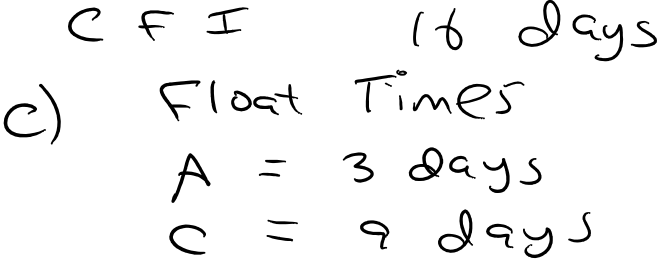
\includegraphics[width=5.5in,height=1.89583in]{media/image4.png}

\textbf{Figure 11.2} Dilbert's ethical dilemma. (Dilbert © United
Feature Syndicate. Reprinted by permission.)

A framework for considering decisions is shown in the 2x2 matrix shown
in Figure 11.3 {[}Die00{]}. The idea is that decisions have both ethical
and legal dimensions to them. The legality may be in terms of internal
company policies or local, state, and federal laws. Quadrant I decisions
are clearly to be avoided as they are not legal or ethical. Quadrant II
decisions present an interesting dilemma since they are legal, but yet
are not ethical. Making such a decision may not have punitive
ramifications, but will have a negative impact on your professional
reputation. Quadrant III decisions certainly feel right and are
tempting, since they are moral but not legal. It is in Quadrants II and
III where most moral dilemmas take place. Taken together, II and III
represent opportunities for reform, to change the system positively so
that ethical choices are legal and unethical choices are illegal. Left
uncorrected, both lead to cynicism with the system, whether it is
company policy or the legal system. Correcting them may take longer to
address than the immediate dilemma, but have the potential for high
payoff. Clearly, quadrant IV decisions are best and the goal in the
decision process.

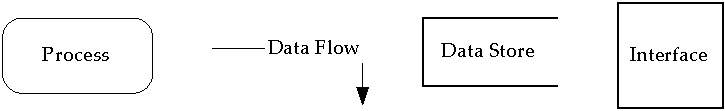
\includegraphics[width=2.48958in,height=2.29167in]{media/image5.emf}

\textbf{Figure 11.3} A 2x2 matrix for ethical decision making
{[}Die00{]}.

One way to evaluate a decision is through what is known as the
\emph{newspaper test}. The idea is to ask whether you would be
comfortable if the decision were published in a newspaper for all to
see. Advice from trusted friends or colleagues can be valuable, but if
they are impacted by the decision, they may not be a good source. Many
companies have an ethics office that provides guidance to which
employees can turn. The IEEE and Online Ethics Center for Engineering
and Science co-sponsor an ethics help-line at
\href{http://www.OnlineEthics.org}{www.OnlineEthics.org}, where ethical
questions can be submitted.

There may be situations in which you are put in an ethical dilemma by
your employer that cannot be resolved internally. As a last resort, you
may go outside of the company to the press or a government agency to
report the problem. This is known as being a
\emph{\textbf{whistleblower}}. An example of this is the space shuttle
Challenger accident, in which the explosion was caused by O-ring
failures in the booster rockets made by Morton-Thiokol. The engineers
and scientists recommended against the launch, but their superiors at
NASA and Morton-Thiokol went ahead over their objections. The engineers
later ``blew the whistle'' by going public with this information.
Although it was too late to avert the disaster, it was valuable in
revealing what had happened and preventing future mishaps. The following
criteria should be satisfied when considering becoming a whistleblower
{[}Deg81{]}:

\begin{itemize}
\item
  The harm to the public must be considerable or serious.
\item
  Concerns must have been made to your superiors (up to the CEO) without
  satisfactory resolution.
\item
  You have documented evidence that would convince an impartial observer
  that your company is wrong. You should have clear technical
  information to support your claims.
\item
  Release of the information outside of the company will prevent the
  harm.
\end{itemize}

Whistleblowing does have risks, particularly loss of job, but the risks
may be well worth it. The Sarbanes-Oxley Act of 2002 improved federal
protection of whistleblowers in the wake of corporate scandals in the
1990s.

\subsection{Case Study Analysis}\label{case-study-analysis}

A good way to develop decision-making skills is by examining case
studies. We now go through the steps of analyzing a case study,
employing the IEEE Code of Ethics as a guide. In order to do so, we
apply a paradigm that is a modification of the one used by Lockheed
Martin Corporation in their employee ethics training programs
{[}Loc97{]}. The modified paradigm is as follows:

\begin{enumerate}
\def\labelenumi{\arabic{enumi}.}
\item
  \emph{Gather information}. What things are known about the situation,
  but also very importantly, what isn't known, and what assumptions are
  being made?
\item
  \emph{Identify the stakeholders.} Who will be affected by the
  decision? They may include you, your company, your supervisors, your
  professional colleagues, your profession, the public, and users of
  your products.
\item
  \emph{Consider what ethical values are relevant to this situation.}
  Identify the elements of the IEEE Code of Ethics and legal issues that
  apply to the situation.
\item
  \emph{Determine a course of action.} Identify different alternative
  decisions and actions. Select the one that you believe best meets the
  interests of the stakeholders and the ethical values.
\end{enumerate}

Example 11.1 demonstrates the application of this paradigm to a case
study for a flawed chip design. More case studies are provided in the
end of chapter problems.

\textbf{Example 11.1} Ethics case study for a flawed chip design. (Texas
A\&M Ethics Case studies, \url{http://ethics.tamu.edu}. Reprinted by
permission.)

Your company has designed a chip for a new scientific calculator that
features high-precision floating-point accuracy to 17 significant digits
for all 250 mathematical functions provided. After one-and-a-half years
in development, and after shipping over 500 beta units to key customers,
the company discovers a problem with certain calculations. In addition,
the company has manufactured 5000 more calculators with this chip that
are ready to be shipped.

In order to expedite floating­ point operations (used in handling
scientific notation in mathematical operations) in a computer or
calculator, certain tables of values often are used to assist in the
speed of execution. (For example, a calculator requiring as long as 3
minutes to perform a tangent calculation would have no market appeal.)
These tables can contain up to 100 integer entries. During beta testing,
you discover that several of these values were incorrectly entered
before burning them into the firmware.

Further testing concludes that because of the location and use of these
table errors, the only mathematical results affected will occur in the
13\textsuperscript{th} to the 17\textsuperscript{th} significant digits
for the double­ precision floating point operations. Your management is
applying subtle pressure to release the chips due to the time and money
invested in the project so far. Identify a plan of action.

\emph{\textbf{\ul{Discussion:}}}

\ul{Step 1: Gather information}

The information makes it clear that the calculator may fail if precision
beyond the 13\textsuperscript{th} digit is needed. What is not known is
the standard precision of a calculator. An Internet search of calculator
specifications was conducted, and it was found that most scientific
calculators have a 10 or 12-digit display plus two digits for the power.
Going to the 13\textsuperscript{th} digit implies a higher than normal
precision calculator. A calculator with 17 significant digits would
likely be used by scientists and engineers for high precision
calculations.

\ul{Step 2: Identify stakeholders}

The following are possible stakeholders:

\begin{itemize}
\item
  Users of the calculator. In certain situations, the user can make an
  incorrect calculation.
\item
  Public. The users of calculator may perform calculations that could
  impact safety of public. This could be a real possibility given the
  likely users.
\item
  Company and employees. There are negative ramifications of releasing a
  faulty product. This could result in monetary harm to the employees of
  the company that you work for.
\end{itemize}

\ul{Step 3: Identify relevant ethical values}

Values from the IEEE Code are identified with a discussion of why they
apply:

1: Release of the faulty calculator has the potential to endanger the
safety of the public.

3: Need to be honest in stating claims as to the precision of the
calculator.

9: There is clear potential to injure the reputation of the company and
its employees.

In terms of legal issues, the company would be opening itself to claims
of negligence, particularly since the defect was identified prior to
release of the product.

\ul{Step 4: Determine a course of action}

Three possible courses of action are:

A: Release the product as is without notifying the customers. This is
not a good choice due to the potential harm to the safety of the public.
This would not pass the newspaper test. It also may be illegal if the
calculator is advertised to work to 17 significant digits.

B: Use the chips in a different calculator that is only guaranteed to
compute at a lower precision, if such an option exists. The company
would have to be producing one, and the technology would have to be
compatible.

C: Throw away the chips and take a loss on their production and correct
the problem. Conduct testing again to verify that the corrected chips
work properly.

Options B and C are both reasonable choices. Option B reduces economic
losses, but acceptance testing should be conducted to make sure they
operate properly at the lower precision. Option C is the safest
solution. Option A might be seen as a viable choice, however, since it
could be reasoned that handheld calculators are not often used for
safety critical applications. That is a risky assumption and the
potential negative effects are great. Also note that the ideal situation
would have been to develop a test plan (Chapter 7) that would have
caught this error before release.

\subsection{Project Application: Incorporating Ethics in the Design
Process}\label{project-application-incorporating-ethics-in-the-design-process}

There are good design practices that can be followed to minimize the
chances that a product will be unsafe. The first and most important
issue is to identify safety and health factors that impact the system
and address them in the design. Its importance is reflected clearly as
the first item in the IEEE Code of Ethics. It is a fundamental canon in
virtually all professional engineering ethical codes. Be aware that
there are often tradeoffs between economic and safety constraints and
one may be satisfied at the expense of the other. It is also important
to follow good practices throughout the design process. Ways that
ethical considerations are included throughout the design process are:

\begin{itemize}
\item
  \emph{Conduct research so that prior art is understood}. This will
  minimize conflicts over intellectual property ownership.
\item
  \emph{Make sure that the requirements meet the needs of the
  stakeholders}. If they do not, the wrong system will be designed. This
  is the concept of validation that was addressed in Chapter 3. Be
  honest and realistic in making claims about what the system can do and
  realize that all have limitations. There is often tension between
  engineering and marketing functions of an organization, with engineers
  often believing that marketing is overstating the capabilities of the
  product. A properly developed Requirements Specification is an
  effective tool for communicating the proposed system functionality to
  all parties.
\item
  \emph{Identify and apply safety standards}. There are many codes and
  guidelines that address safety in design for particular technologies.
  They should be identified and applied as necessary. For example, it
  may be wise to design a consumer product to meet UL (Underwriter's
  Laboratory) guidelines. It may difficult to fully incorporate
  guidelines in a capstone design project, depending upon the complexity
  of the design and the standards. However, consideration should be
  given to identifying those that apply.
\item
  \emph{Keep the design space large and explore as many solutions as
  possible}. The hallmark of design is that there is typically no single
  solution to the problem, but many that may \emph{\textbf{satisfice}.}
  Satisfice means that a solution may meet the design requirements, but
  may not be the optimal solution. It is important to fully understand
  the technical tradeoffs involved in a given design and their impact on
  health and safety.
\item
  \emph{Consider all of the possible ways that a system can fail.} This
  follows the IEEE Code of Ethics, which indicates that engineers should
  understand technology, its application, and potential consequences.
  This can be done formally through the use of techniques such as
  failure mode analysis and the examination of system reliability
  (Chapter 8). In safety critical systems, the use of redundant systems
  may be warranted to improve reliability. An excellent example of a
  technical design that incorporates redundancy in a safety critical
  application for a hot tub controller is found in the article
  \emph{Designing for Reliability, Maintainability, and Safety} by
  George Novacek in \ul{Circuit Cellar} magazine {[}Nov00, Nov01{]}.
\item
  \emph{Identify ways in which the system can fail by misuse or operator
  error}. This requires thinking like a beginner who is completely
  unfamiliar with the technology. Provide manuals for operation and
  safety labels where appropriate.
\item
  \emph{Make realistic cost and project schedule estimates}. The IEEE
  Code of Ethics indicates that engineers should be honest and realistic
  in stating claims, and this applies to the project plan as well as the
  system cost.
\item
  \emph{Conduct design reviews}. The purpose of a design review is to
  have peers who are knowledgeable about the design and the technology
  conduct a review of the work you have done. This can be a humbling,
  but valuable, experience. It is also in keeping with the IEEE Code of
  Ethics, which indicates that engineers should seek, accept, and offer
  honest criticism of technical work and acknowledge and correct errors.
\item
  \emph{Verify the engineering requirements during testing}. We saw in
  Chapter 3 that verification is the process of showing that the system
  is built properly. Verification usually occurs at the end of a project
  at a time that there may be a great deal of pressure to complete the
  tests and finish the project.
\end{itemize}

\subsection{Summary and Further
Reading}\label{summary-and-further-reading}

This chapter provided a brief overview of ethics, morality, and
different ethical decision making systems. The IEEE Code of Ethics was
presented, which serves as a set of ethical values for the electrical
and computer engineering profession and provides a basis for analyzing
ethical dilemmas. Legal issues surrounding intellectual property and
product liability were provided. Advice for incorporating safety and
ethics in design projects was provided as well as a paradigm for
analyzing case studies.

The background on ethical frameworks and its importance in engineering
came from a number of articles. The article \emph{What has Ethics to do
with me?: I am an Engineer} {[}Gob99{]} provides background on
rule-based ethics, universality, and transitivity. \emph{A Piercian
Approach to Professional Ethics Instruction} {[}Cha02b{]} addressed
ethical decision-making frameworks. \emph{Ethical Considerations in the
Engineering Design Process} {[}Van01{]} emphasizes the need to keep the
design space as large as possible. The article \emph{Integrating Ethics
and Design} {[}Mcl93{]} does a good job of describing three different
levels of ethical decision making in technical, professional, and social
contexts. The two engineering design textbooks by Dieter {[}Die00{]} and
Hyman {[}Hym98{]} are good resources on legal and intellectual property
issues. The United States Patent and Trademark Office has an excellent
website (\href{http://www.uspto.gov}{www.uspto.gov}) with information on
patents, applying for a patent, and a searchable patent database. The
website \href{http://www.HowStuffWorks.com}{www.HowStuffWorks.com} is
also a good source on ethical theory, patents, and legal issues
surrounding product liability.

\subsection{Problems}\label{problems}

\begin{enumerate}
\def\labelenumi{\arabic{enumi}.}
\item
  Describe the relationship between ethics and morals.
\item
  Describe the differences between morals and values.
\item
  Which patent is most relevant for engineering inventions, a design
  patent or utility patent? Why?
\item
  What are the criteria that are used in evaluating patents?
\item
  Explain the importance of claims in a patent application.
\item
  Discuss the tradeoffs involved between using patents and trade secrets
  to protect intellectual property.
\item
  When can reverse-engineering be used, and how can the information
  obtained from it be used?
\item
  What is the difference between negligence and strict liability in tort
  law?
\item
  For the case study presented below, apply the ethical decision making
  paradigm presented in Section 11.5 to analyze the situation. Present
  potential solutions to the scenario and provide a discussion of them.
\end{enumerate}

\begin{quote}
\ul{\hfill\break
Case Study: Disk Drive Diagnostics. (Copyright John Wallberg. Reprinted
by permission.)}

SCSI, an industry standard system for connecting devices (like disks) to
computers, provides a vendor ID protocol by which the computer can
identify the supplier (and model) of every attached disk.

Company C makes file servers consisting of a processor and disks. Disks
sold by C identify C in their vendor ID. Disks from other manufacturers
can be connected to C\textquotesingle s file servers; however, the file
server software performs certain maintenance functions, notably
pre-failure warnings based on performance monitoring, only on C-supplied
disks.

Company P decides to compete with C by supplying cheaper disks for
C\textquotesingle s file server. They quickly discover that while their
disks work on C\textquotesingle s file servers, their disks lack a
pre-failure warning feature that C\textquotesingle s disks have.
Therefore, the CEO of P directs you, the engineer in charge of the disk
product, to find a solution to the problem of no pre-failure warning for
your disks. Using reverse engineering, you discover that by changing the
vendor ID of P's disks, the C file servers will treat P disks as C
disks. Your management at company P instructs you to incorporate this
change into your product so that you can advertise the disks as ``100\%
C-compatible.'' What would you do in this situation?
\end{quote}

\begin{enumerate}
\def\labelenumi{\arabic{enumi}.}
\setcounter{enumi}{9}
\item
  For the case study presented below, apply the ethical decision making
  paradigm presented in Section 11.5 to analyze the situation. Present
  potential courses of action and provide a discussion of them.
\end{enumerate}

\begin{quote}
\ul{Case Study: Encryption Software} (Texas A\&M Ethics Case Studies,
\url{http://ethics.tamu.edu}. Reprinted by permission.)

You are a recently hired engineer who has been recruited directly out of
college. For your first assignment, your boss asked you to write a piece
of software to provide security from "prying eyes" over e­mailed
documents; these documents would be used internally by the company. This
software will subsequently be distributed to different departments.

Upon completion of this software project, you saw a program on the local
news about an individual in California who has made similar software
available overseas. This individual is currently under prosecution in a
federal court for the distribution of algorithms and information which
(by law) must remain within the United States for purposes of national
security.

It occurs to you that your company is a multinational corporation and
that the software might have been distributed overseas. You then
discover that the software has indeed been sent overseas to other
offices within the corporation. You speak with your boss, informing him
of the news program from the night before. He shrugs off this comment,
stating that ``The company is based in the United States and we are
certainly no threat to national security in any way. Besides,
there\textquotesingle s no way anyone will find out about software we
use internally.''

You agree with your boss, and let it go. Later on however, you receive a
letter from a gentleman working as a contractor for his company
overseas. Through some correspondence regarding the functionality of the
software and technical matters, you learn that the Middle Eastern office
had been supplying his software outside the company to contractors and
clients so that they could exchange secure e­mailed documents. What would
you do in this situation?
\end{quote}

\begin{enumerate}
\def\labelenumi{\arabic{enumi}.}
\setcounter{enumi}{10}
\item
  For the case study presented below, apply the ethical decision making
  paradigm presented in Section 11.5 to analyze the situation. Present
  potential courses of action and provide a discussion of them.
\end{enumerate}

\begin{quote}
\ul{Case Study: A Failure.} (Texas A\&M Ethics Case Studies,
\url{http://ethics.tamu.edu}. Reprinted by permission.)

You work for Velky Measurement which has for years provided DGC
Corporation with sophisticated electronic equipment for patient health
monitoring systems. Recently, DGC returned a failed piece of measurement
equipment. A meeting was held with representatives of Velky and DGC to
discuss the problem. This included you and your project manager who is
intimately acquainted with the returned equipment. During the course of
the meeting it becomes apparent to you that the problem has to be
Velky\textquotesingle s. You suspect that the equipment failed because
of an internal design problem and that it was not properly tested.
However, at the conclusion of the meeting your project manager
represents Velky's official position---the test equipment is functioning
properly.

You keep silent during the meeting, but afterwards talk to your project
manager about his diagnosis. You suggest that Velky tell DGC that the
problem is due to a design fault and that Velky will replace the
defective equipment. You manager replies, ``\emph{I
don\textquotesingle t think it\textquotesingle s wise to acknowledge
that it\textquotesingle s our fault. There\textquotesingle s no need to
hang out our wash and lessen DGC\textquotesingle s confidence in the
quality of our work. A good will gesture to replace the equipment should
suffice}.''

Utlimately, Velky's management replaces the equipment because DGC has
been such a good customer. Although Velky replaces the equipment at its
own expense, it does not disclose the real nature of the problem. What
would you do in this situation?
\end{quote}

\begin{enumerate}
\def\labelenumi{\arabic{enumi}.}
\setcounter{enumi}{11}
\item
  For the case study presented below, apply the ethical decision making
  paradigm presented in Section 11.5 to analyze the situation. Present
  potential courses of action and provide a discussion of them.
\end{enumerate}

\begin{quote}
\ul{Case Study: A Vacation} (Texas A\&M Ethics Case Studies,
\url{http://ethics.tamu.edu}. Reprinted by permission.)

You work for Rancott and were looking forward to an upcoming trip for
weeks. Once you were assigned to help install Rancott's equipment for
Boulding Corporation, you arranged a vacation at a nearby ski resort.
The installation was scheduled to be completed on the
12\textsuperscript{th} and your vacation would begin on the
13\textsuperscript{th}. That meant a full week of skiing with three of
your old college buddies.

Unfortunately, not all of the equipment arrived on time. Eight of the
ten identical units were installed by mid-morning on the
12\textsuperscript{th}. Even if the remaining two units had arrived that
morning, it would take another full day to install them. However, you
were informed that it might take as long as two more days for the units
to arrive.

``\emph{Terrific,}'' you sighed, ``\emph{there goes my vacation---and
all the money I put down for the condo}.'' ``\emph{No problem},''
replied Jerry, the Boulding engineer who had worked side-by-side with
you as each of the first eight units was installed. He said ``\emph{I
can handle this for you. We did the first eight together.
It\textquotesingle s silly for you to have to hang around and blow your
vacation}.'' Jerry knew why you were sent to supervise the installation
of the new equipment. It had to be properly installed in order to avoid
risking injuries to those who use it. Although you are aware of this,
you are confident that Jerry is fully capable to supervise the
installation of the remaining two units. What would you do?
\end{quote}

\textbf{Concept Generation}
